\documentclass[11pt, oneside]{article} 
\usepackage[utf8]{inputenc}
  	% use "amsart" instead of "article" for AMSLaTeX format
\usepackage{geometry}                		% See geometry.pdf to learn the layout options. There are lots.
\geometry{letterpaper}                   		% ... or a4paper or a5paper or ... 
%\geometry{landscape}                		% Activate for for rotated page geometry
%\usepackage[parfill]{parskip}    		% Activate to begin paragraphs with an empty line rather than an indent
\usepackage{graphicx}				% Use pdf, png, jpg, or eps§ 
\usepackage{amssymb}
\usepackage{multicol}


\title{Rapport du projet : Benchmark}
\author{Charles Jacquet & Stéphane Kimmel}

\begin{document}

\begin{multicols}{2}

\section{Introduction}
Le but de ce projet-ci était de déterminé la rapidité d'une machine en faisant des appels aux fonctions systèmes en language mais aussi et surtout, comparer le temps d'exécution des différentes fonctions systèmes entre elles.  \\
En effet, chaque fonction système coute du temps et le but était entre autre de comparer le temps mis par la combinaison de deux fonctions systèmes par rapport à l'appel d'une seule fonction système réalisant la même chose.

\section{Choix d'implementations}
\subsection{Readdir}
L'appel de la fonction readdir permet de parcourir / lister le contenu d'un dossier. Nous avons donc décidé de comparer le temps mis par readdir pour lire un dossier contenant un nombre croissants de fichiers ainsi qu'un nombre croissants de fichiers remplis. Nous voulions essayer de savoir si readdir prenait plus de temps lorsque les fichiers contenaient une chaine de caractère quelconque. C'est pourquoi, sur l'image ci-dessous, il y a 2 graphiques. \\

\subsection{Writev comparé à 'write' et 'lseek'}
Tout d'abord, il nous a fallu comprendre à quoi servait la fonction writev. Nous nous sommes donc rendu compte qu'elle permettait d'écrire un ensemble de buffers l'un à la suite des autres. Pour ce faire, il fallait créer un tableau de structure iov, dont chaque structure possède le buffer (iov\_base) et également la taille sur laquelle il faut écrire ce buffer (iov\_len). C'est pourquoi nous avons décidé de prendre comme sénario, de stocker des données sur des secteurs. Pour ce faire, nous avons utilisé un même buffer tout au long par facilité mais on pourrait imaginer par exemple de laisser assez de place pour stocker des structures ou tout autre chose. De plus comme taille de secteur, ici, nous avons choisi une taille égale au double de la taille de la chaine de caractères.
Ensuite, il nous suffisait de mesurer le temps grâce aux fonctions du benchmark pour exécuter writev ainsi que fsync pour s'assurer que le temps mesuré contient bien l'écriture du buffer dans le fichier.
Nous devions aussi faire la même chose avec write et lseek. Pour ce faire, il nous fallait d'abord, grâce à lseek, déplacer l'offset du descripteur de fichier pour le mettre au début de la bonne section. Ensuite, on pouvait écrire le buffer grâce à write et fsync de nouveau pour s'assurer de l'écriture du buffer.
Ensuite pour pouvoir bien comparer les deux, nous recommençons l'opération un certain nombre de fois et à chaque fois on écrit un buffer de plus.

\section{Interpretation des résultats}
\subsection{Readdir}
Voici le graphique obtenu en sortie après l'exécution du benchmark \\
\includegraphics[scale=0.35]{readdir.png}
\\
Nous pouvons clairement apercevoir une suite de segments de longueur horizontale de 125 fichiers qui s'élèvent de plus en plus. 
De plus, nous pouvons remarquer que les espaces verticaux entre ces segments sont équivalent, que ce soit lorsque les fichiers sont pré-alloués avec une certaine taille ou non. 
En effet, après multiples recherches sur internet, cela serait dû au fait que readdir est appellé réellement 1 fois tous les 125 (les sources divergent sur ce nombre) fichiers et
qu'il ne fait que charger les attributs de chaque fichier ensuite avec getattr. Une fois qu'il atteint 125 appels à getattr, il rappelle readdir. Ceci expliquerait assez bien l'allure du graphe de notre benchmark.

\subsection{Writev}

\begin{center}

%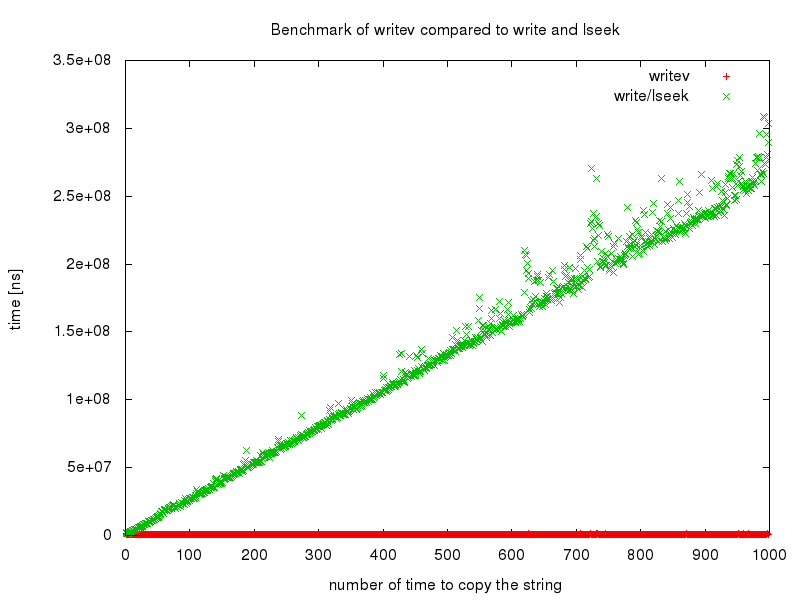
\includegraphics[scale=0.2]{writev.png}

\end{center}
On peut facilement se rendre compte que writev est beaucoup plus rapide que la combinaison de write et lseek. De plus, nous avons fait les test avec uniquement Writev et write pour pouvoir comparer et il était déjà clair que writev était bien plus rapide. Ensuite nous avions au début oublier de faire un fsync. Lorsque nous l'avons implémenté, nous avons vu une différence énorme pour les deux temps. Nous en avons tiré comme conclusion que ce qui prenait du temps, c'est bien l'appel système d'écriture dans le fichier. Nous émettons donc l'hypothèse que writev, forme un buffer qu'il va ensuite écrire en un minimum de fois pour limiter le nombre d'appel qui prennent vraiment du temps, c'est-à-dire l'appel qui permet d'écrire dans un fichier (qui de plus est un appel bloquant).


\section{Conclusion}
Au final, ce projet-ci aura été le plus enrichissant car il s'agissait de comprendre réellement ce qu'il y a derrière les fonctions systèmes elles-mêmes pour comprendre leurs temps d'exécution respectifs. Par contre, ce projet n'aura pas été de tout repos, les premiers problèmes se posant dès la compilation du fork que l'on a fait du git. Pas mal d'autres problèmes de liens sont apparus çar notre projet devait s'intégrer dans un projet déjà conçu. De plus, pour rajouter nos deux fonctions personnelles au benchmark, il aura fallu ouvrir et comprendre la plupart des fichiers du projet donné afin d'en adapter certains. 
\end{multicols}
\end{document}  